\documentclass{article}
\usepackage{cmap}
\usepackage[utf8]{inputenc}
\usepackage[english,ukrainian]{babel}
\usepackage{graphicx}
\usepackage{geometry}
\usepackage{listings}
\usepackage{float}
\usepackage{multicol}
\geometry{
	a4paper,
	left=20mm,
	right=20mm,
	top=20mm,
	bottom=20mm
}
\lstset{
	language=c,
	tabsize=4,
	keepspaces,
	showstringspaces=false,
	breaklines,
}
\graphicspath{ {./pictures} }
\setlength{\parindent}{4em}

\newcommand\subject{Алгоритми та структури даних}
\newcommand\lecturer{доцент кафедри ПЗ\\Коротєєва Т.О.}
\newcommand\teacher{асистент кафедри ПЗ\\Франко А.В.}
\newcommand\mygroup{ПЗ-22}
\newcommand\lab{11}
\newcommand\theme{Алгоритм пошуку КМП}
\newcommand\purpose{Навчитися застосовувати алгоритм пошуку КМП при розв’язуванні задач та перевірити його ефективність на різних масивах даних. Експериментально визначити складність алгоритму}

\begin{document}
	\begin{normalsize}
		\begin{titlepage}
			\thispagestyle{empty}
			\begin{center}
				\textbf{МІНІСТЕРСТВО ОСВІТИ І НАУКИ УКРАЇНИ\\
					НАЦІОНАЛЬНИЙ УНІВЕРСИТЕТ "ЛЬВІВСЬКА ПОЛІТЕХНІКА"}
			\end{center}
			\begin{flushright}
				Інститут \textbf{КНІТ}\\
				Кафедра \textbf{ПЗ}
			\end{flushright}
			\vspace{200pt}
			\begin{center}
				\textbf{ЗВІТ}\\
				\vspace{10pt}
				До лабораторної роботи № \lab\\
				\textbf{На тему}: “\textit{\theme}”\\
				\textbf{З дисципліни}: “\subject”
			\end{center}
			\vspace{112pt}
			\begin{flushright}
				
				\textbf{Лектор}:\\
				\lecturer\\
				\vspace{28pt}
				\textbf{Виконав}:\\
				
				студент групи \mygroup\\
				Коваленко Д.М.\\
				\vspace{28pt}
				\textbf{Прийняв}:\\
				
				\teacher\\
				
				\vspace{28pt}
				«\rule{1cm}{0.15mm}» \rule{1.5cm}{0.15mm} 2022 р.\\
				$\sum$ = \rule{1cm}{0.15mm}……………\\
				
			\end{flushright}
			\vspace{\fill}
			\begin{center}
				\textbf{Львів — 2022}
			\end{center}
		\end{titlepage}
		
		\begin{description}
			\item[Тема.] \theme.
			\item[Мета.] \purpose.
		\end{description}
		
		\section*{Лабораторне завдання}

	Розробити програму, яка:
		\begin{center}
			2.       Задано два тексти. В першому тексті знайти найкоротше слово і знайти його входження в другий текст відповідним алгоритмом пошуку.
		\end{center}
		
		\section*{Теоретичні відомості}
		Маємо масив символів S з n елементів (текст) та масив P з m - взірець. Необхідно знайти перше входження взірця в масив. Схема алгоритму полягає у поступовому порівнянні взірця з текстом та зсуву по тексту на кількість співпавших символів у разі знайденого неспівпадіння. Алгоритм використовує просте спостереження, що коли відбувається неспівпадіння тексту і взірця, то взірець містить у собі достатньо інформації для того, щоб визначити де наступне входження може початися, таким чином пропускаючи кількаразову перевірку попередньо порівняних символів. Попередньо проводиться дослідження взірця та для кожного його підрядка визначається префікс-суфікс-функція. Для цього вираховується найдовший початок підрядка, який співпадає з його кінцем.
		
		Алгоритм КМП
		
		КМП 1. Встановити і=0.
		
		КМП 2. j=0, d=1.
		
		КМП 3. Поки j<m, i<n
		
		Перевірка: якщо S[i]=P[j], то d++, i++.j++ поки d != m.
		
		КМП 4. Інакше встановити зсув взірця на d-D[d] позицій по тексту . Перейти на крок КМП 2.
		
		КМП 5. Кінець.
		
		\section*{Хід роботи}
		\begin{lstlisting}[language=C]
    fn first_indexof_needle<N: AsRef<[u8]>>(&self, needle: N) -> Option<usize> {
	let needle = needle.as_ref();
	let pattern_table = Self::pattern_table(needle);
	let haystack = &self.as_ref();
	
	if needle.is_empty() {
		return Some(0);
	}
	
	let mut s: usize = 0;
	let mut i: usize = 0;
	
	loop {
		if i >= needle.len() {
			println!("Found '{}': ..{}..", from_utf8(&needle).unwrap(), from_utf8(&haystack[s.checked_sub(3).unwrap_or(0)..usize::min(s+needle.len()+3, haystack.len())]).unwrap());
			return Some(s);
		}
		if s + i >= haystack.len() {
			println!("Not found");
			return None;
		}
		if needle[i] == haystack[s + i] {
			println!("{} == {}", needle[i] as char, haystack[s + i] as char);
			i += 1;
		} else {
			println!("{} != {}", needle[i] as char, haystack[s + i] as char);
			match pattern_table[i] {
				0 => {
					println!("shift {}", std::cmp::max(1, i));
					s += std::cmp::max(1, i);
					i = 0;
				}
				prefix_len => {
					println!("shift {}", std::cmp::max(1, i));
					s += i - prefix_len;
					i = prefix_len;
				}
			}
		}
	}
}

		\end{lstlisting}
		
		\begin{figure}[H]
			\centering
			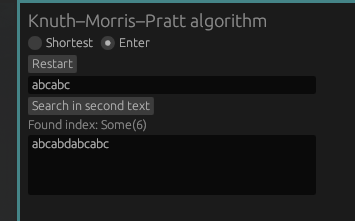
\includegraphics[scale=0.7]{1}
			\caption{Вигляд програми}
		\end{figure}
		
		\begin{figure}[H]
			\centering
			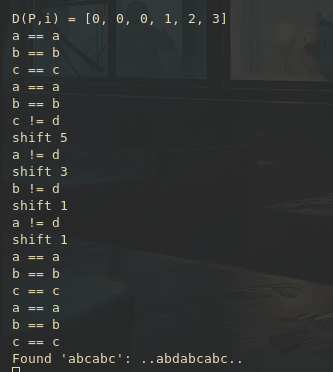
\includegraphics[scale=0.7]{2}
			\caption{Покроковий вивід}
		\end{figure}
		
		\section*{Висновоки}
		Під час виконання лабораторної роботи я навчився застосовувати алгоритм пошуку KMP при розв’язуванні задач та перевірити його ефективність на різних масивах даних. Експериментально визначив складність алгоритму. 
		
	\end{normalsize}
\end{document}
